\chapter{Applications}


\section{BayesCNN for Image Classification}
And now I begin my third chapter here \dots

And now to cite some more people~\citet{Rea85,Ancey1996}

\section{BayesCNN for Image Super Resolution}

The task referred as Super Resolution is the recovery of a High Resolution image from a given Low Resolution image. It is applicable to many areas like medical imaging \citet{10.1007/978-3-642-40760-4_2}, face recognition \citet{1203152} and so on.

There are many ways to do a single image super resolution and a detailed benchmarks of the methods is provided by Yang \citet{Yang2014SingleImageSA}. Mainly there are four major ways to do it:\\
Prediction Models. SISR algorithms in this category generate HR images
from LR inputs through a predefined mathematical formula without training
data. Interpolation-based methods (bilinear, bicubic, and Lanczos) generate HR
pixel intensities by weighted averaging neighboring LR pixel values. Since interpolated intensities are locally similar to neighboring pixels, these algorithms generate good smooth regions but insufficient large gradients along edges and at high-frequency regions. The IP method [16] exploits a predefined downsampling model from a HR image to a LR image. Given an initial HR image, this method iteratively generates a LR image through the predefined downsampling
model and compensates the difference map in LR back to the HR image. Since
a generated HR image is designed to best match the LR input image under the
linear downsampling model, the contrast along edges is better enhanced than
the results generated by bicubic interpolation.\\

Edge Based Methods. Edges are important primitive image structures that
play a prime role in visual perception. Several SISR algorithms have been proposed to learn priors from edge features for reconstructing HR images. Various edge features have been proposed such as the depth and width of an edge [8] or the parameter of a gradient profile [30]. Since the priors are primarily learned from edges, the reconstructed HR images have high-quality edges with proper sharpness and limited artifacts. However, edge priors are less effective for modeling other high-frequency structures such as textures.\\

Patch Based Methods. Given a set of paired LR and HR training images,
patches can be cropped from the training images to learn mapping functions.]. In addition to equally averaging overlapped patches, several methods for blending overlapped pixels have been proposed including weighted averaging [11,44], Markov Random Fields [10], and Conditional Random Fields [38].



The global \ac{SR} problem assumes \ac{LR} data to be a low-pass filtered (blurred), downsampled and noisy version of \ac{HR} data. It is a highly ill-posed problem, due to the loss of high-frequency information that occurs during the non-invertible low-pass filtering and subsampling operations. Furthermore, the SR operation is effectively a one-to-many mapping from \ac{LR} to \ac{HR} space which can have multiple solutions, of which determining the correct solution is non-trivial. A key assumption that underlies many \ac{SR} techniques is that much of the high-frequency data is redundant and thus can be accurately reconstructed from low frequency components. \ac{SR} is therefore an inference problem, and thus relies on our model of the statistics of images in question.


\subsection{Our Work}

We build our work upon Shi \citet{DBLP:journals/corr/ShiCHTABRW16} work that shows that performing Super Resolution work in High Resolution space is not the optimal solution and it adds the computation complexity. We used a Bayesian Convolutional Neural Network to extract features in the Low Resolution space. We use an efficient sub-pixel convolution layer, as proposed by \citet{DBLP:journals/corr/ShiCHTABRW16}, which learns an array of upscaling filters to upscale the final Low Resolution feature maps into the High Resolution output. This replaces the handcrafted bicubic filter in the Super Resolution pipeline with more complex upscaling filters specifically trained for each feature map, and also reduces the computational complexity of the overall Super Resolution operation.

\begin{figure*}[htbp]
\begin{center}
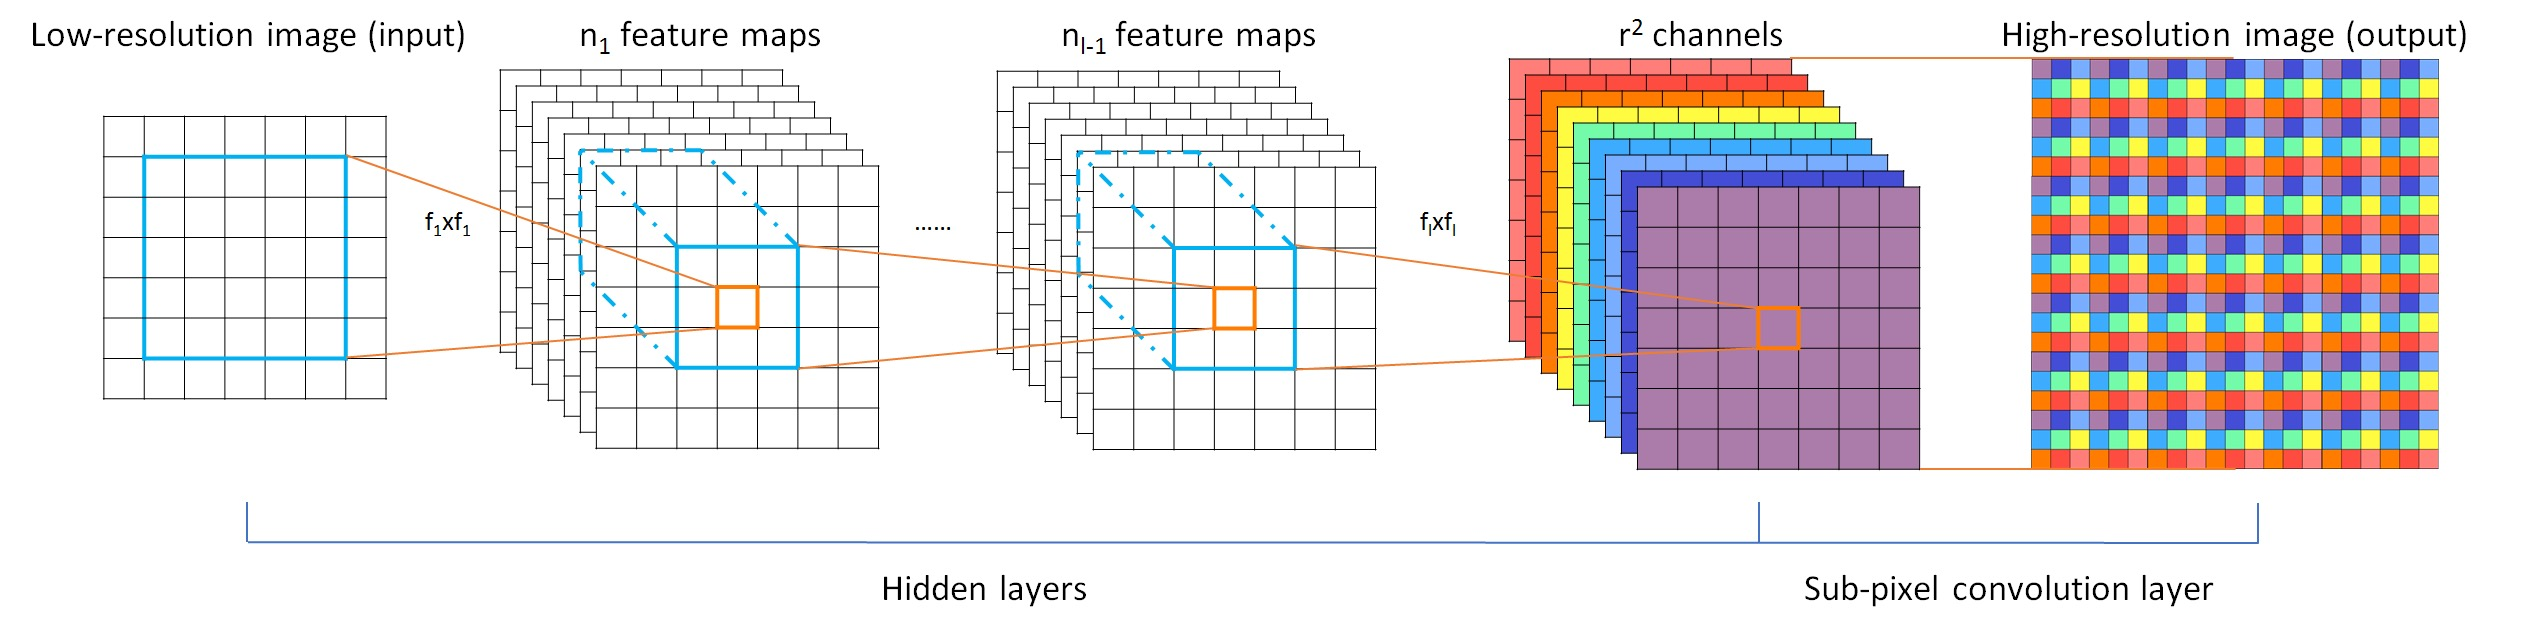
\includegraphics[width=1.0\linewidth]{Chapter6/Figs/networkstructure.jpg}
\caption{The proposed efficient sub-pixel convolutional neural network (ESPCN), with two convolution layers for feature maps extraction, and a sub-pixel convolution layer that aggregates the feature maps from \ac{LR} space and builds the \ac{SR} image in a single step.}
\label{fig:networkstructure}
\end{center}
\end{figure*}

\subsubsection{Empirical Analysis}



\section{BayesCNN for Generative Adversarial Networks}

\section{Introduction}

Learning reusable feature representations from large unlabeled datasets has been an area of active research. In the context of computer vision, one can leverage the practically unlimited amount of unlabeled images and videos to learn good intermediate representations, which can then be used on a variety of supervised learning tasks such as image classification. We propose that one way to build good image representations is by training Generative Adversarial Networks (GANs) \citep{Goodfellow2014}, and later reusing parts of the generator and discriminator networks as feature extractors for supervised tasks. GANs provide an attractive alternative to maximum likelihood techniques. One can additionally argue that their learning process and the lack of a heuristic cost function (such as pixel-wise independent mean-square error) are attractive to representation learning. GANs have been known to be unstable to train, often resulting in generators that produce nonsensical outputs. There has been very limited published research in trying to understand and visualize what GANs learn, and the intermediate representations of multi-layer GANs.

In this paper, we make the following contributions
\begin{itemize}  
    \item We propose and evaluate a set of constraints on the architectural topology of Convolutional GANs that make them stable to train in most settings. We name this class of architectures Deep Convolutional GANs (DCGAN)
    \item We use the trained discriminators for image classification tasks, showing competitive performance with other unsupervised algorithms.
    \item We visualize the filters learnt by GANs and empirically show that specific filters have learned to draw specific objects.
    \item We show that the generators have interesting vector arithmetic properties allowing for easy manipulation of many semantic qualities of generated samples.
\end{itemize}

\section{Related Work}
\subsection{Representation Learning from unlabeled data}
Unsupervised representation learning is a fairly well studied problem in general computer vision research, as well as in the context of images. A classic approach to unsupervised representation learning is to do clustering on the data (for example using K-means), and leverage the clusters for improved classification scores. In the context of images, one can do hierarchical clustering of image patches \citep{coates2012learning} to learn powerful image representations. Another popular method is to train auto-encoders (convolutionally, stacked \citep{vincent2010stacked}, separating the what and where components of the code \citep{zhao2015stacked}, ladder structures \citep{rasmus2015semi}) that encode an image into a compact code, and decode the code to reconstruct the image as accurately as possible. These methods have also been shown to learn good feature representations from image pixels. Deep belief networks \citep{lee2009convolutional} have also been shown to work well in learning hierarchical representations.

\subsection{Generating natural images}

Generative image models are well studied and fall into two categories: parametric and non-parametric.

The non-parametric models often do matching from a database of existing images, often matching patches of images, and have been used in texture synthesis \citep{efros1999texture}, super-resolution \citep{freeman2002example} and in-painting \citep{hays2007scene}.

Parametric models for generating images has been explored extensively (for example on MNIST digits or for texture synthesis \citep{portilla2000parametric}). 
However, generating natural images of the real world have had not much success until recently. A variational sampling approach to generating images \citep{kingma2013auto} has had some success, but the samples often suffer from being blurry. Another approach generates images using an iterative forward diffusion process \citep{sohl2015deep}. Generative Adversarial Networks \citep{Goodfellow2014} generated images suffering from being noisy and incomprehensible. A laplacian pyramid extension to this approach \citep{denton2015deep} showed higher quality images, but they still suffered from the objects looking wobbly because of noise introduced in chaining multiple models. A recurrent network approach \citep{gregor2015draw} and a deconvolution network approach \citep{dosovitskiy2014learning} have also recently had some success with generating natural images. However, they have not leveraged the generators for supervised tasks.







    
\fbox{
    \parbox{\textwidth}
    {
        Architecture guidelines for stable Deep Convolutional GANs
        \begin{itemize}
            \item Replace any pooling layers with strided convolutions (discriminator) and fractional-strided convolutions (generator).
            \item Use batchnorm in both the generator and the discriminator.
            \item Remove fully connected hidden layers for deeper architectures.
            \item Use ReLU activation in generator for all layers except for the output, which uses Tanh.
            \item Use LeakyReLU activation in the discriminator for all layers.
        \end{itemize}
    }
}
